\documentclass[12pt, titlepage]{article}

\usepackage{fullpage}
\usepackage[round]{natbib}
\usepackage{multirow}
\usepackage{booktabs}
\usepackage{tabularx}
\usepackage{graphicx}
\usepackage{float}
\usepackage{hyperref}
\hypersetup{
    colorlinks,
    citecolor=blue,
    filecolor=black,
    linkcolor=red,
    urlcolor=blue
}

%% Comments

\usepackage{color}

\newif\ifcomments\commentstrue %displays comments
%\newif\ifcomments\commentsfalse %so that comments do not display

\ifcomments
\newcommand{\authornote}[3]{\textcolor{#1}{[#3 ---#2]}}
\newcommand{\todo}[1]{\textcolor{red}{[TODO: #1]}}
\else
\newcommand{\authornote}[3]{}
\newcommand{\todo}[1]{}
\fi

\newcommand{\wss}[1]{\authornote{blue}{SS}{#1}} 
\newcommand{\plt}[1]{\authornote{magenta}{TPLT}{#1}} %For explanation of the template
\newcommand{\an}[1]{\authornote{cyan}{Author}{#1}}

%% Common Parts

\newcommand{\progname}{Flick Picker}
\newcommand{\authname}{Team 7, 7eam
\\ Talha Asif - asift
\\ Jarrod Colwell - colwellj
\\ Madhi Nagarajan - nagarajm
\\ Andrew Carvalino - carvalia    
\\ Ali Tabar - sahraeia
}     

\usepackage{hyperref}
    \hypersetup{colorlinks=true, linkcolor=blue, citecolor=blue, filecolor=blue,
                urlcolor=blue, unicode=false}
    \urlstyle{same}
                                


\newcounter{acnum}
\newcommand{\actheacnum}{AC\theacnum}
\newcommand{\acref}[1]{AC\ref{#1}}

\newcounter{ucnum}
\newcommand{\uctheucnum}{UC\theucnum}
\newcommand{\uref}[1]{UC\ref{#1}}

\newcounter{mnum}
\newcommand{\mthemnum}{M\themnum}
\newcommand{\mref}[1]{M\ref{#1}}

\begin{document}

\title{System Design for \progname{}} 
\author{\authname}
\date{\today}

\maketitle

\pagenumbering{roman}

\section{Revision History}

\begin{tabularx}{\textwidth}{p{3cm}p{2cm}X}
\toprule {\bf Date} & {\bf Version} & {\bf Notes}\\
\midrule
January 18 & 1.0 & Added content to section 6.4, some potential content to 6.1 - Jarrod \\
January 18 & 1.1 & Completed Sections 3, 4, 6.1, 6.2, 6.4 - Jarrod \\
January 18 & 1.2 & Completed Sections 5, 6.3, 8, 12 - Madhi \\
January 18 & 1.3 & Editing and adding to reflection - All \\

\bottomrule
\end{tabularx}

\newpage

\section{Reference Material}

This section records information for easy reference.

\subsection{Abbreviations and Acronyms}

\renewcommand{\arraystretch}{1.2}
\begin{tabular}{l l} 
  \toprule		
  \textbf{symbol} & \textbf{description}\\
  \midrule 
  \progname & A program to find Movies, TV Shows, or Anime for individuals or groups\\
  UI & User Interface\\
  MG & Module Guide\\
  MIS & Module Interface Specification\\
  API & Application Programming Interface\\
  \bottomrule
\end{tabular}\\

\newpage

\tableofcontents

\newpage

\listoftables

\listoffigures

\newpage

\pagenumbering{arabic}

\section{Introduction}
\hspace*{14pt} In order to continue with the implementation of Flick Picker, it is important to create a System Design document. This will help in outlining the design decisions that were made so as to not cause confusion and increased work in the implementation process. It is also important to outline the tasks, both in regard to the work that needs to be done and with whom the work has been assigned. This document, including these design decisions and timeline, will be complimented by the MG and the MIS to further outline the specifications of Flick Picker. 

\section{Purpose}
\hspace*{14pt} The purpose of this design documentation is to cover the behaviour of our system under a variety of conditions, detail the components of the system, discuss any connections between design choices and the requirements, user interface designs, and a timeline of when tasks should be complete and who should be completing them. Information in this design document should support or further explain the information found in the MG and MIS.

\section{Scope}

The system will allow the user to interact with the application, in order to find appropriate Movie/Anime recommendations for themselves and/or their group. The system will also allow the user to securely login and manage their user profile and their groups. External APIs are also made use of to retrieve movie and anime data.

\begin{figure}[H]
	\centering
	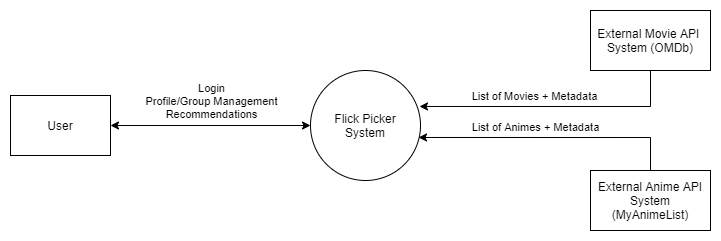
\includegraphics[width=0.8\textwidth]{SystemContext.png}
	\caption{System Context of the entire system and its environment}
	\label{FigUH}
\end{figure}

\section{Project Overview}

\subsection{Normal Behaviour}
\begin{itemize}
	\item \textbf{Native Login Module:} Provided the email and password, this module will communicate with the database module to authorize or deny the user's login.
	\item \textbf{OAuth Login Module:} Provided the authorization from an OAuth login, this module will communicate with the database module to authorize the user's login or account creation.
	\item \textbf{Database Module:} Communicates with the database to verify logins, store Movie, TV Show, and Anime data, and to retrieve user data.
	\item \textbf{Profile Module:} Communicates with the Database module to get a user's information to provide to the UI. Allows for users to add friends and create or join groups. 
	\item \textbf{Friends Module:} Allows for users to see their friends, accept friend invites, and invite their friends to groups. 
	\item \textbf{Group Module:} Compiles preferences of users and sends this information to the Matching Algorithm Module. Presents the received recommendations to the users of the group. 
	\item \textbf{Matching Algorithm Module:} Receives the set of preferences and queries the API Module using these preferences to create a set of Movies, TV Shows, and/or Anime recommendations. Sends this set of recommendations back to the group module. 
	\item \textbf{API Module:} Queries external APIs daily for the most popular Movies, TV Shows, and Anime. Sends this information to the database. Receives query calls from the Matching Algorithm Module and returns information to it. 
\end{itemize}

\subsection{Undesired Event Handling}
\begin{itemize}
	\item \textbf{API Module - No Match Found:} If the Matching Algorithm queries the API Module and it cannot find Movies, TV Shows, or Anime that match the filters, the API module will send requests to the external APIs with these filters. 
	\item \textbf{Various Modules - Rate Limiting:} If an individual attempts to overload the system with certain requests, they will be timed out via rate limiting.
\end{itemize}

\subsection{Component Diagram}
\begin{figure}[H]
	\centering
	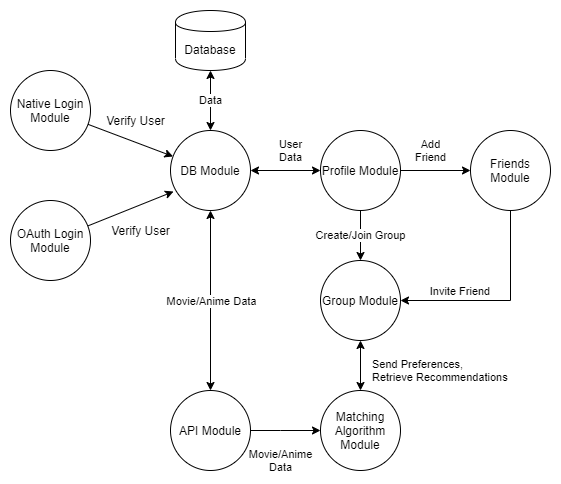
\includegraphics[width=0.7\textwidth]{ComponentDiagram.png}
	\caption{Component Diagram showing all modules}
	\label{FigUH}
\end{figure}

\subsection{Connection Between Requirements and Design} \label{SecConnection}

\subsubsection{Connection Between Authentication Requirements and Design}
\hspace*{14pt} For email and password authentication, the user's email and a hashed form of their password are stored in the database. Upon login request, the inputted email and password will be compared to the pairs in the database and the login will either succeed or fail depending on whether a match is found. 

Google and Facebook OAuth will provide authorization and an email to Flick Picker which will have / create an account with this email. If an account with this email already exists using OAuth, the user is logged in successfully. If an account using the previous method (email and password) exists, the user will be prompted to login using their email and password as above. If an account with this email does not exist, the user will be logged in and a new OAuth account will be created. They will then be brought to the new user page (creation of username, preferences, etc.). 

Upon clicking the logout button, the user will be brought to the login screen and their token is removed.

\subsubsection{Connection Between Profile/Group Requirements and Design}
\hspace*{14pt} There will be a page for users to modify their information, including username and password if the account is not an OAuth account. Additionally, there will be a page for users to access and modify their preferences (e.g. genre, show type, etc.). A separate page will enable users to create and join groups. Group invites will be provided through the invited user's email or friends page. The owner of a group can view the group members, join requests, and other information regarding group management on the group management page. 

\subsubsection{connection Between Recommendation Requirements and Design}
\hspace*{14pt} Daily, Flick Picker will retrieve information about the top 3000 most popular Movies, TV Shows, and Anime and store that information for quick access. This information will be used in the vast majority of all recommendations. If a recommendation cannot be found within these Movies, TV Shows, or Anime, additional queries will be sent to the relevant APIs to find a recommendation.

During the recommendation process for a group, individual users reflect their desire to watch a recommendation using the 'like', 'neutral', or 'dislike' buttons. This information will be stored alongside their preferences to aid in future recommendations for both the group and the individuals. 

Given user permission, Flick Picker will send emails to all members in a group once a recommendation has been chosen. 

\section{System Variables}

\subsection{Monitored Variables}
N/A

\subsection{Controlled Variables}
N/A

\subsection{Constants Variables}
N/A

\section{User Interfaces}

Mockups of the user interface were designed in Figma. Below are the mockups, organized by the module they fall under.

\begin{figure}[H]
	\centering
	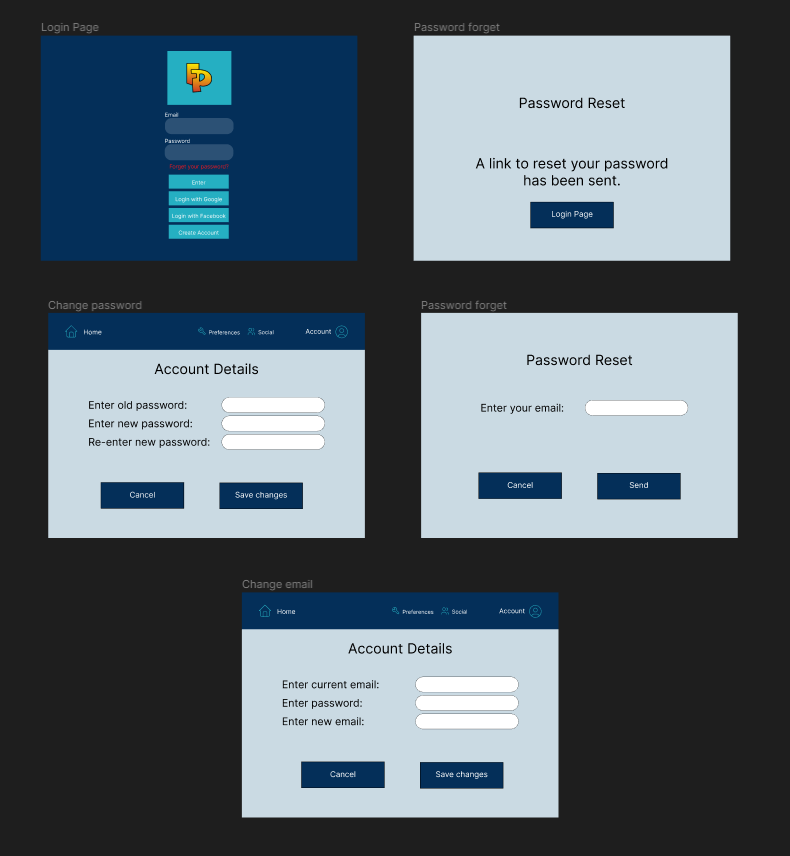
\includegraphics[width=0.9\textwidth]{figma/login.png}
	\caption{UI mockups of the Login Module. Note that both the Native Login Module and Auth Module are represented in the Login Page}
	\label{FigUH}
\end{figure}

\begin{figure}[H]
	\centering
	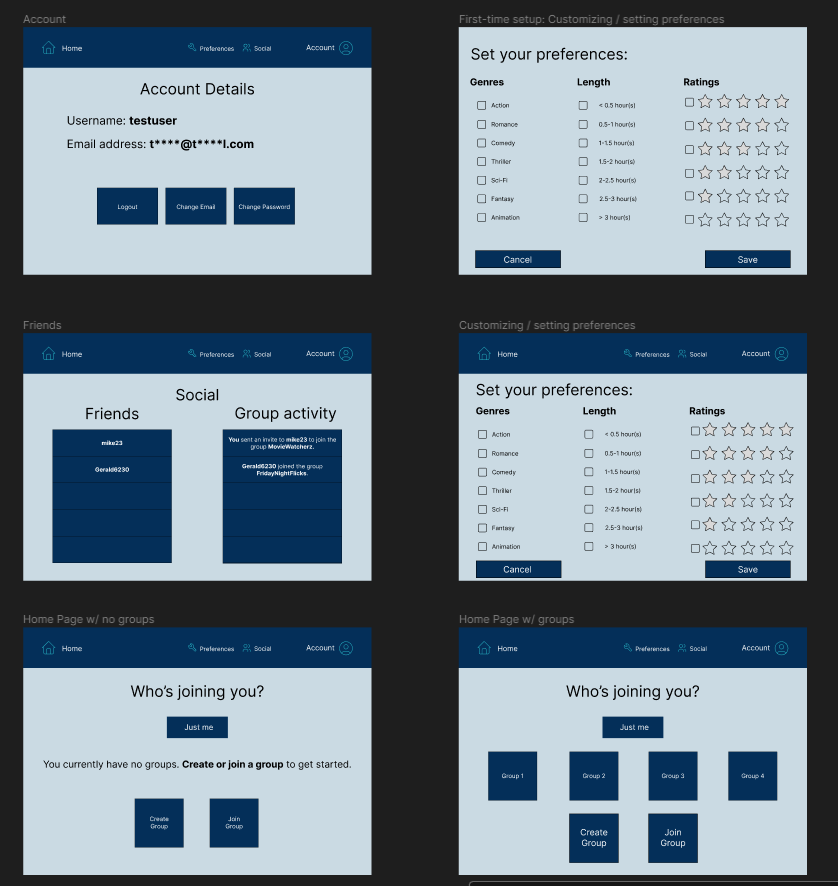
\includegraphics[width=0.9\textwidth]{figma/profile.png}
	\caption{UI mockups of the Profile \& Friend Modules}
	\label{FigUH}
\end{figure}

\begin{figure}[H]
	\centering
	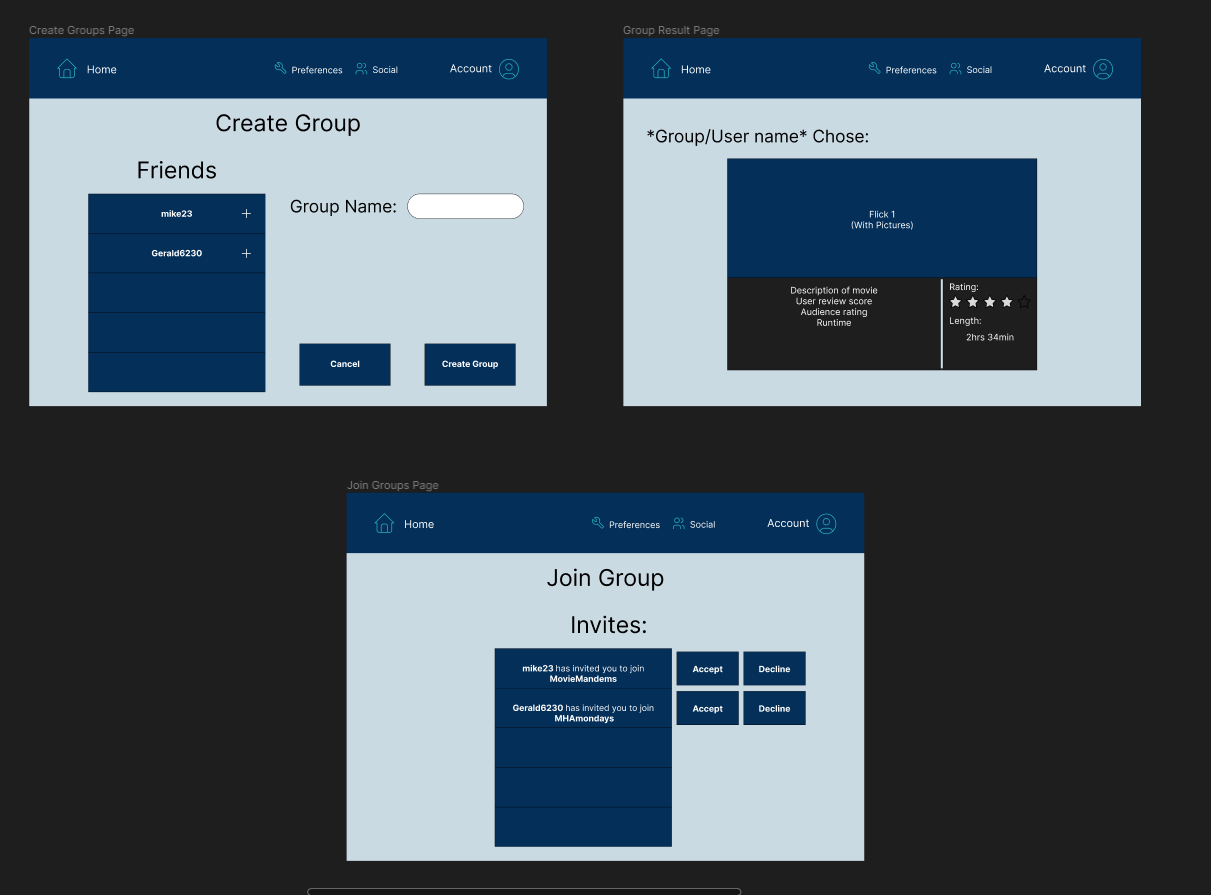
\includegraphics[width=1\textwidth]{figma/groups.png}
	\caption{UI mockups of the Group Module}
	\label{FigUH}
\end{figure}

\begin{figure}[H]
	\centering
	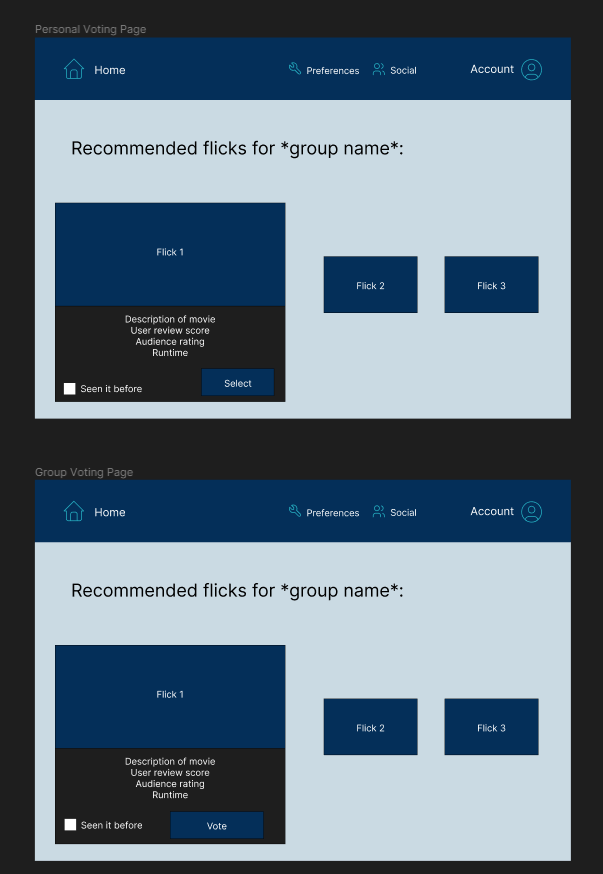
\includegraphics[width=0.7\textwidth]{figma/voting.png}
	\caption{UI mockups of the Matching Algorithm Module}
	\label{FigUH}
\end{figure}



\section{Design of Hardware}
N/A

\section{Design of Electrical Components}
N/A

\section{Design of Communication Protocols}
N/A

\section{Timeline}
\begin{tabularx}{\textwidth}{|X|p{4cm}|p{2cm}|p{2cm}|}
	\hline
	{\bf Task} & {\bf Module} & {\bf Task Due Date} & {\bf Assigned To} \\
	\hline
	Create Login \& Password Reset Pages & Login (Native \& Auth) & Jan 23 & Talha\\
	\hline
	Integrate External APIs to backend & API & Jan 23 & Madhi\\
	\hline
	Setup Firebase DB & API, DB & Jan 23 & Jarrod\\
	\hline
	Create Home \& Profile Pages & Profile & Jan 25 & Andrew\\
	\hline
	Create Preference Pages & Profile & Jan 25 & Ali\\
	\hline
	Add native login functionality & Native Login & Jan 30 & Jarrod\\
	\hline
	Add Auth functionality & Auth Login & Jan 30 & Madhi\\
	\hline
	Create Groups Page & Group & Feb 2 & Ali\\
	\hline
	Create Friends Page & Friend & Feb 2 & Andrew\\
	\hline
	Create Recommendation Pages & Friend & Feb 3 & Talha\\
	\hline
	Hookup Backend to Frontend & All & Feb 5 & Talha, Jarrod\\
	\hline
	Deploy Frontend and Backend & All & Feb 12 & Madhi\\
	\hline
	Manual Testing & All & continuous & Team\\
	\hline
	Integration Tests & All & Feb 15 & Team\\
	\hline
\end{tabularx}

% \bibliographystyle {plainnat}
% \bibliography{../../../refs/References}

\newpage{}

\appendix

\section{Interface}

\wss{Include additional information related to the appearance of, and
interaction with, the user interface}

\section{Mechanical Hardware}
N/A

\section{Electrical Components}
N/A

\section{Communication Protocols}
N/A

\section{Reflection}

The information in this section will be used to evaluate the team members on the
graduate attribute of Problem Analysis and Design.  Please answer the following questions:

\begin{enumerate}
  \item What are the limitations of your solution?  Put another way, given
  unlimited resources, what could you do to make the project better? (LO\_ProbSolutions)
  \item Give a brief overview of other design solutions you considered.  What
  are the benefits and tradeoffs of those other designs compared with the chosen
  design?  From all the potential options, why did you select documented design?
  (LO\_Explores)
\end{enumerate}

\subsection{Group Reflection}
1. Our solution's two most significant limitations are the number of developers and time constraints. As 7eam only has five developers with solely software engineering experience, we need to learn how to market a product. We also need multiple years of development experience to avoid pitfalls that individuals who have worked in the industry would know to avoid. If we were given an unlimited number of individuals to make an entire development team with dedicated teams per dev-op, frontend, backend, and business teams, the application would see a much more significant influx of users and have an incredibly refined design. Furthermore, we are constrained by time, not just by the due dates but by how much content we five individual developers can put in. We could refine the application incredibly well with infinite time and no other resources. 
	
Outside of those limitations, the APIs also proved to be limiting. There are some ideas that the team had that we were unable to go through with due to the lacking APIs, especially on the Anime side of things. If these APIs were available or if this information magically appeared in our database, we could have developed a more complex algorithm and potentially some cool new features. 
	
2. Another design solution was a minor decision about pairing users and preferences together. The benefit is that they go hand-in-hand, where users are directly linked to their preferences. The downside being it adds an overhead to updating the preferences list, and since we are going to take into account user feedback for the preferences, it could go through a handful of updates. Therefore splitting it off into a module in isolation and linking the user is a safer implementation.

Another design decision that we ended up not going with was to have, alongside each preference, a scale to say how important that preference is to a user, potentially on a scale of 1-10 or 1-3. We felt like this would help people who might not care much about the type of entertainment (Movie, TV Show, Anime) in comparison to the genre (e.g. they really love action and comedy but hate romance). Ultimately this idea was placed on a potential addition list since it doesn't add enough value to the system in comparison to the complication it poses to both the users and the developers. 

\end{document}